\NeedsTeXFormat{LaTeX2e}
\documentclass[a4paper,12pt,
headsepline,           % Linie zw. Kopfzeile und Text
oneside,               % einseitig
pointlessnumbers,      % keine Punkte nach den letzten Ziffern in Überschriften
bibtotoc,              % LV im IV
%DIV=15,               % Satzspiegel auf 15er Raster, schmalere Ränder   
%BCOR15mm              % Bindekorrektur
%,draft
]{scrartcl}

\usepackage{amsmath}
\usepackage{amsfonts}
\usepackage{amssymb}
\usepackage{enumitem}
\usepackage[utf8]{inputenc} % this is needed for umlauts
\usepackage[ngerman]{babel} % this is needed for umlauts
\usepackage[T1]{fontenc} 
\usepackage{commath}
\usepackage{xcolor}
\usepackage{booktabs}
\usepackage{float}
\usepackage{tikz-timing}
\usepackage{tikz}
\usepackage{multirow}
\usepackage[final]{pdfpages}
\usepackage{blindtext}
\usepackage[scaled]{helvet}
\usepackage{hyperref}
\usepackage{comment}
\usepackage{mathtools}
\DeclarePairedDelimiter{\ceil}{\lceil}{\rceil}

\usetikzlibrary{calc,shapes.multipart,chains,arrows}

\KOMAoptions{DIV=last} % Neuberechnung Satzspiegel nach Laden von Paket helvet

\usepackage{scrpage2}
\pagestyle{useheadings}

\renewcommand{\familydefault}{\sfdefault} 

\setlength{\parindent}{0pt}   % kein linker Einzug der ersten Absatzzeile
\setlength{\parskip}{1.4ex plus 0.35ex minus 0.3ex} % Absatzabstand, leicht variabel

\newcommand{\fullname}{Gruppe 10}
\newcommand{\titel}{Endabnahmedokument}
\newcommand{\jahr}{2018/2019}
\newcommand{\dozent}{Florian Ege}
\newcommand{\betreuer}{Stefanos Mytilineos}
\newcommand{\fakultaet}{Ingenieurwissenschaften, Informatik und\\Psychologie}
\newcommand{\institut}{Institut für Softwaretechnik und Programmiersprachen}

\pdfinfo{
    /Author (\fullname)
    /Title (\titel)
    /Producer     (pdfeTex 3.14159-1.30.6-2.2)
    /Keywords ()
}

\hypersetup{
    pdftitle=\titel,
    pdfauthor=\fullname,
    pdfsubject={Softwaregrundprojekt-Abgabe},
    pdfproducer={pdfeTex 3.14159-1.30.6-2.2},
    colorlinks=false,
    pdfborder=0 0 0	% keine Box um die Links!
}

% Trennungsregeln
\hyphenation{Sil-ben-trenn-ung}


\newcommand{\begriff}[7] {
	\begin{table}[H]
		\centering
		\begin{tabular}{|p{2,5cm}|p{12cm}|}
			%\hline
			%\toprule \\
			\hline
			\textbf{Begriff} & \textbf{#1} \\ \hline
			%\midrule \\
			\textbf{Beschreibung} & #2 \\ \hline
			%\midrule
			\textbf{Ist-ein} & #3 \\ \hline
			%\midrule
			\textbf{Kann-sein} & #4 \\ \hline
			%\midrule
			\textbf{Aspekt} & #5 \\ \hline
			%\midrule
			\textbf{Bemerkung} & #6 \\ \hline
			%\midrule
			\textbf{Beispiel} & #7 \\ %\hline
			%\bottomrule
			\hline
		\end{tabular}
	\end{table}
}

\newcommand{\anf}[7] {
    \begin{table}[H]
        \centering
        \begin{tabular}{|p{3.2cm}|p{11.3cm}|}
        	\hline
            \textbf{ID:} & \textbf{#1} \\ \hline
            \textbf{Titel:} & #2 \\ \hline
            \textbf{Beschreibung:} & #3 \\ \hline
            \textbf{Begründung:} & #4 \\ \hline
            \textbf{Abhängigkeiten:} & #5 \\ \hline
            \textbf{Priorität:} & #6 \\ \hline
            \textbf{Akteure:} & #7 \\ \hline
        \end{tabular}
    \end{table}
}

\newcounter{fanfCount}
\newcommand{\fanf}[6] {
    \stepcounter{fanfCount}
    \anf{FA\thefanfCount}{#1}{#2}{#3}{#4}{#5}{#6}
}
\newcounter{qanfCount}
\newcommand{\qanf}[6] {
    \stepcounter{qanfCount}
    \anf{QA\theqanfCount}{#1}{#2}{#3}{#4}{#5}{#6}
}

\newcommand{\akt}[4] {
    \begin{table}[H]
        \centering
        \begin{tabular}{|p{3cm}|p{11.5cm}|}
        	\hline
            \textbf{ID:} & \textbf{#1} \\ \hline
            \textbf{Titel:} & #2 \\ \hline
            \textbf{Beschreibung:} & #3 \\ \hline
            \textbf{Rolle:} & #4 \\ \hline
        \end{tabular}
    \end{table}
}

\newcounter{faktCount}
\newcommand{\fakt}[3] {
    \stepcounter{faktCount}
    \akt{AKT\thefaktCount}{#1}{#2}{#3}
}

\begin{document}
    \thispagestyle{empty}
    \begin{addmargin*}[4mm]{-10mm}

        
\includegraphics[height=1.8cm]{images/unilogo_bild}
        \hfill
        
\includegraphics[height=1.8cm]{images/unilogo_wort}\\[1em]

        {\footnotesize
        %{\bfseries Universität Ulm} \textbar ~89069 Ulm \textbar ~Germany
        \hspace*{115mm}\parbox[t]{35mm}{\bfseries Fakultät für\\
        \fakultaet\\
        \mdseries \institut}\\[2cm]

        \parbox{140mm}{\bfseries \LARGE \titel}\\[2.5em]
        {\footnotesize Softwaregrundprojekt an der Universität Ulm}\\[3em]

        {\footnotesize \bfseries Vorgelegt von:}\\
        {\footnotesize \fullname\\}\\ [1em]
        {\footnotesize \bfseries Dozent:}\\
        {\footnotesize \dozent\\}\\[1em]
        {\footnotesize \bfseries Betreuer:}\\
        {\footnotesize \betreuer}\\ [1em]
        {\footnotesize \jahr}
        }
    \end{addmargin*}
    \pagebreak
    \tableofcontents
    \pagebreak

    \section{Verwendete Technologien}
    \subsection{Server und KI}
\subsubsection{Buildtools und Frameworks}
Der Server und die KI wurden in C++17 geschrieben.
Als Compiler wurde dafür der GNU-C++-Compiler (GCC) (Version 8.3, Lizenziert unter GPLv3) verwendet,
als Buildsystem wurde CMake (Version 3.10, Lizenziert unter BSD-3) in Kombination mit GNU Make (Version 4.1, Lizenziert unter GPLv3) genutzt.

\subsubsection{Statische Analyse und Tests}
Zur statischen Codeanalyse wurde Clang-Tidy (Version 6.0, Lizenziert unter Apache 2) verwendet,
als weiteres Tool zur Codeanalyse wurde der Sonar-Scanner (Version 3.3.0.1492, proprietär) in Verbindung mit der Community-Edition des Webinterface SonarCloud (\url{https://sonarcloud.io}) genutzt.

Unit- und Mock-Tests wurden mit Google-Test bzw. Google-Mock (Version 2.56, Lizenziert unter BSD-3) implementiert.
Um undefiniertes Verhalten zu vermeiden wurde das Programm während der Ausführung mit Adress Sanitizer (Version 5.0, Lizenziert unter Apache 2) überprüft.

\subsubsection{Dokumenation und Styleguide}
Alle Teile des Quellcodes wurden mithilfe von Doxygen-Kommentaren (Version 1.8, Lizenziert unter GPLv2) dokumentiert.

Es wurde sich während des Entwicklungsprozess an den Linux-Kernel-Styleguide gehalten werden. 
Zwei wesentliche Abweichungen von diesem Styleguide sind eine Einrückungstiefe von 4 Spaces, sowie die Platzierung der öffnenden Klammer bei Funktionsaufrufen in der selben Zeile 
(die Unterscheidung bei der Platzierung von öffnenden geschweiften Klammern ist wohl ursprünglich K\&R zuzuschreiben, die diese Inkonsistenz damit begründen, 
dass Funktionen sich nicht verschachteln lassen, das ist mit C++11 durch Lambdas nicht mehr der Fall).

\subsubsection{Externe Librarys}
Als externe Librarys wurde libwebsockets (Version 3.1.0, LGPLv2, \url{https://github.com/warmcat/libwebsockets}), 
nlohmann::json (Version 3.6.0 bzw. 3.6.1, MIT, \url{https://github.com/nlohmann/json}) sowie MLP (GPLv3, \url{https://github.com/aul12/MLP}) verwendet.

\subsubsection{Tools}
Als Entwicklungsumgebung wurden die IDE CLion (Version 2019.1, proprietär) sowie der Editor vim (Version 8.0, Lizenziert als Careware).

\subsection{Client}

\subsubsection{Framework und Dependencies}
	\paragraph{Vue.js}
	Als Frontend-Framwork wurde Vue.js verwendet, das es u. a. erlaubt, umfangreiche SPAs zu entwickeln (Version 2.6.10, \url{https://vuejs.org/}, mit vue-template-compiler: 2.5.21).
	
	\begin{itemize}
		\item The MIT License (MIT)
	\end{itemize}
	
	\paragraph{Fontawesome}
	Fontawesome bietet eine umfangreiche Sammlung kostenloser SVG-Grafiken zur Gestaltunge von UIs, die sich einfach einbinden und konfigurieren lassen. Weitere Informationen unter: \url{https://fontawesome.com/}\\
	Verwendete Versionen:
	\begin{itemize}
		\item fortawesome/fontawesome-svg-core: 1.2.19
		\item fortawesome/free-solid-svg-icons: 5.9.0
		\item fortawesome/vue-fontawesome: 0.1.6
		\item CC BY 4.0 License
	\end{itemize}
	
	

	\paragraph{Animate.css}
	Animated.css bietet eine Sammlung vorgefertigter CSS-Animationen, die sich einfach in die Anwendung einbinden lassen (Version 3.7.2, \url{https://daneden.github.io/animate.css/}).
	
	\begin{itemize}
		\item The MIT License (MIT)
	\end{itemize}

	\paragraph{Umfassendes JavaScript}
	Mit diesem Package lassen sich auch die neuesten Features von JavaScript bis hin zu ES2018 in die Anwendung integrieren. Babel (siehe unten), erlaubt es dann, diese Features in von allen Browsern unterstütztes JavaScript zu übersetzen (Version 2.6.5, \url{https://www.npmjs.com/package/core-js}).
	
	\begin{itemize}
		\item The MIT License (MIT)
	\end{itemize}

	\paragraph{vuex}
	Vuex ist eine Erweiterung für Vue, die Features für application state management nach dem Vorbild von Redux zur Verfügung stellt (Version 3.1.1, \url{https://vuex.vuejs.org/}).
	
	\begin{itemize}
		\item The MIT License (MIT)
	\end{itemize}

\subsubsection{Dev-Dependencies}
Um den Entwicklungsprozess möglichst produktiv zu gestalten, wurden einige Dev-Dependencies eingesetzt:

	\paragraph{Vue CLI}
	Die Vue CLI erlaubt ein schnelles Setup von neuen Vue-Projketen über die Kommandozeile. Dabei können vorab oder nachträglich über einfache Befehle Konfigurationen vorgenommen werden (Version 3.6.0, \url{https://cli.vuejs.org/}).
	
	\begin{itemize}
		\item The MIT License (MIT)
	\end{itemize}

	\paragraph{ESLint}
	Da JavaScript eine dynamische Programmiersprache ist, kann die Fehlersuche von Zeit zu Zeit recht umständlich sein.
Mit ESLint, einem JavaScript Linter, können viele Fehler (und spezifizierte Stil-Regeln) vorab erkannt bzw. durchgesetzt werden. Hier wird es in Verbindung mit Babel (neuste ECMA Script Syntax-Unterstützung) und Prettier verwendet. Weitere Informationen unter: \url{https://eslint.org/}\\
Verwendete Versionen:
	\begin{itemize}
		\item eslint: 5.16.0
		\item eslint-loader: 2.1.2
		\item eslint-plugin-vue: 5.0.0
		\item eslint-config-prettier: 4.3.0
		\item eslint-plugin-prettier: 3.1.0
		\item babel-eslint: 10.0.1
		\item vue/cli-plugin-eslint: 3.6.0
		\item The MIT License (MIT)
	\end{itemize}

	\paragraph{Babel}
	Babel erlaubt es, die neuesten Features von JavaScript (ECMA Script) zu verwenden, ohne auf eine vollständige Browser-Unterstützung angewiesen zu sein. Babel übersetzt die neuesten Features in Code mit einer von allen Browsern unterstützten Version von ECMA Script (Version 7.4.4, \url{https://babeljs.io/}).
	
	\paragraph{Prettier}
	Prettier ist ein Style Formatter, der hier im Zusammenspiel mit ESLint zum Einsatz kommt. Bei jedem Speichervorgang werden die Style-Guides des Vue-Core-Teams automatisch umgesetzt. Es entsteht eine saubere und einheitliche code base (Version 1.18.2 mit vue/cli-plugin-babel: 3.6.0, \url{https://prettier.io/}).
	
	\begin{itemize}
		\item The MIT License (MIT)
	\end{itemize}
	
	

Das genaue Setup für Linting und Formatierung ist von diesem (\url{https://medium.com/@gogl.alex/how-to-properly-set-up-eslint-with-prettier-for-vue-or-nuxt-in-vscode-e42532099a9c}) Medium-Artikel inspiriert.


\subsubsection{Tools}

	\paragraph{VisualStudio}
Als Texteditor kam für den Client ausschließlich VisualStudio Code zum Einsatz (\url{https://code.visualstudio.com/}).

	\paragraph{Affinity Designer}
Zum Erstellen von Spielgrafiken wurde die kommerzielle Software Affinity Designer v1.7.1 von Serif verwendet (\url{https://affinity.serif.com/de/designer/}).




    
    \section{Projekttagebuch}
    Das Projekttagebuch wurde mit der Hilfe eines Google-Formular verwaltet. Die dazugehörige Eingabemaske ist unter folgendem Link zu finden: \url{https://docs.google.com/forms/d/e/1FAIpQLSdlc-WKKGjKdk1e3qPVxXkzdcqY6LYrXj0sgBuA4_gtZcW2Hw/viewform}\\
Die einzelnen Eintrage sind unter dem nachfolgenden Link einsehbar: \url{https://drive.google.com/open?id=1AJPGgD-9MZZR8e6xCiLpxgbUAKqJjAv-QcIBXes6I5M}\\
Aus diesen Einträgen wurden die folgenden Diagramme automatisch generiert:

\begin{figure}[H]
    \centering
    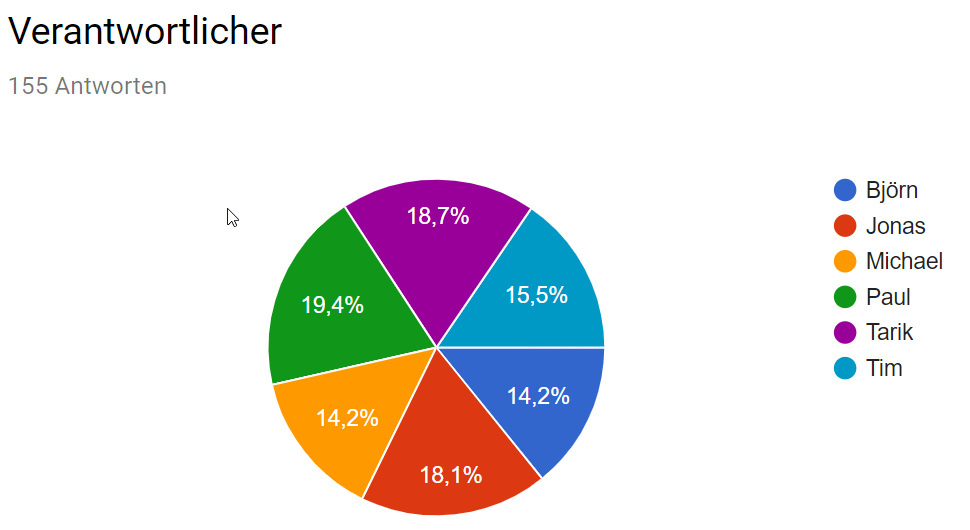
\includegraphics[width=\textwidth]{../Endabnahme/images/Verantwortlicher_Chart.png}
\end{figure}

\begin{figure}[H]
    \centering
    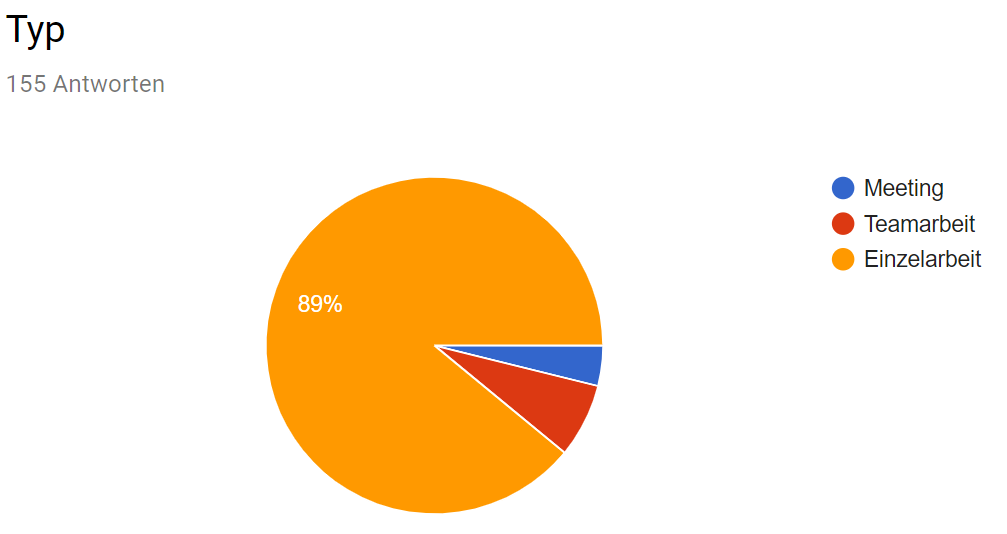
\includegraphics[width=\textwidth]{../Endabnahme/images/Typ_Chart.png}
\end{figure}

\begin{figure}[H]
    \centering
    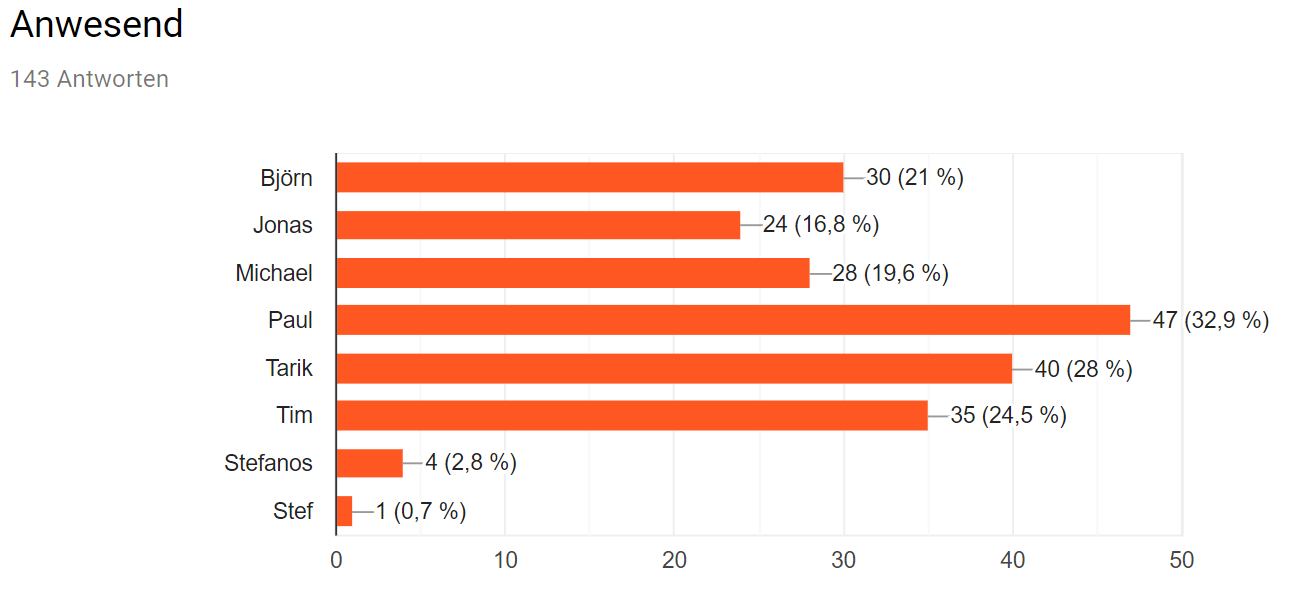
\includegraphics[width=\textwidth]{../Endabnahme/images/Anwesend_Chart.png}
\end{figure}
    
    \section{UML - Komponentendiagramm}
    
\subsection{Komponentendiagramm zum Server}
\begin{figure}[H]
    \centering
    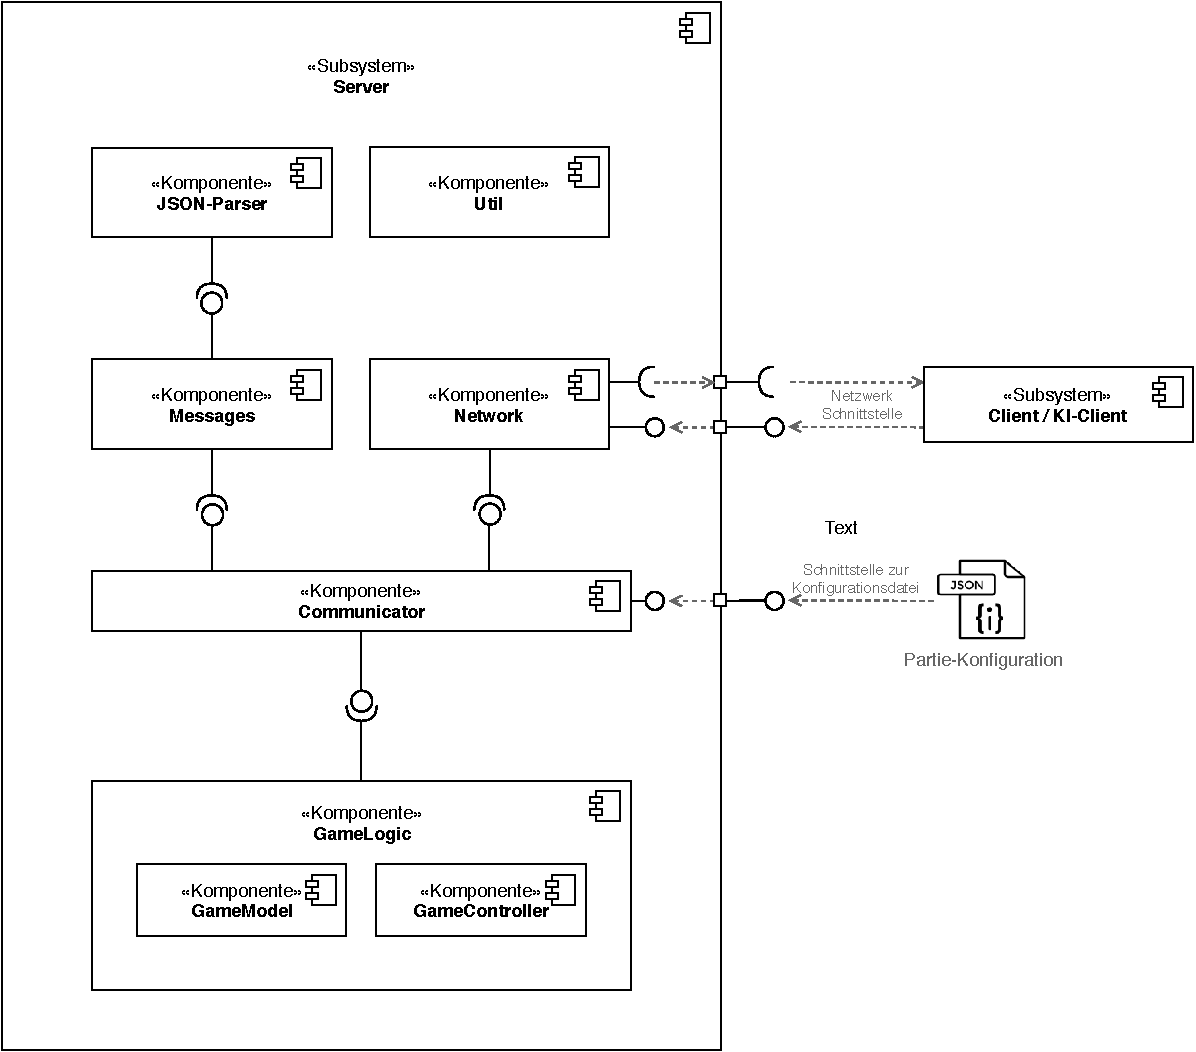
\includegraphics[scale=0.85]{../Endabnahme/images/ServerDiagramme.pdf}
\end{figure}

\subsection{Komponentendiagramm zur KI}
\begin{figure}[H]
    \centering
    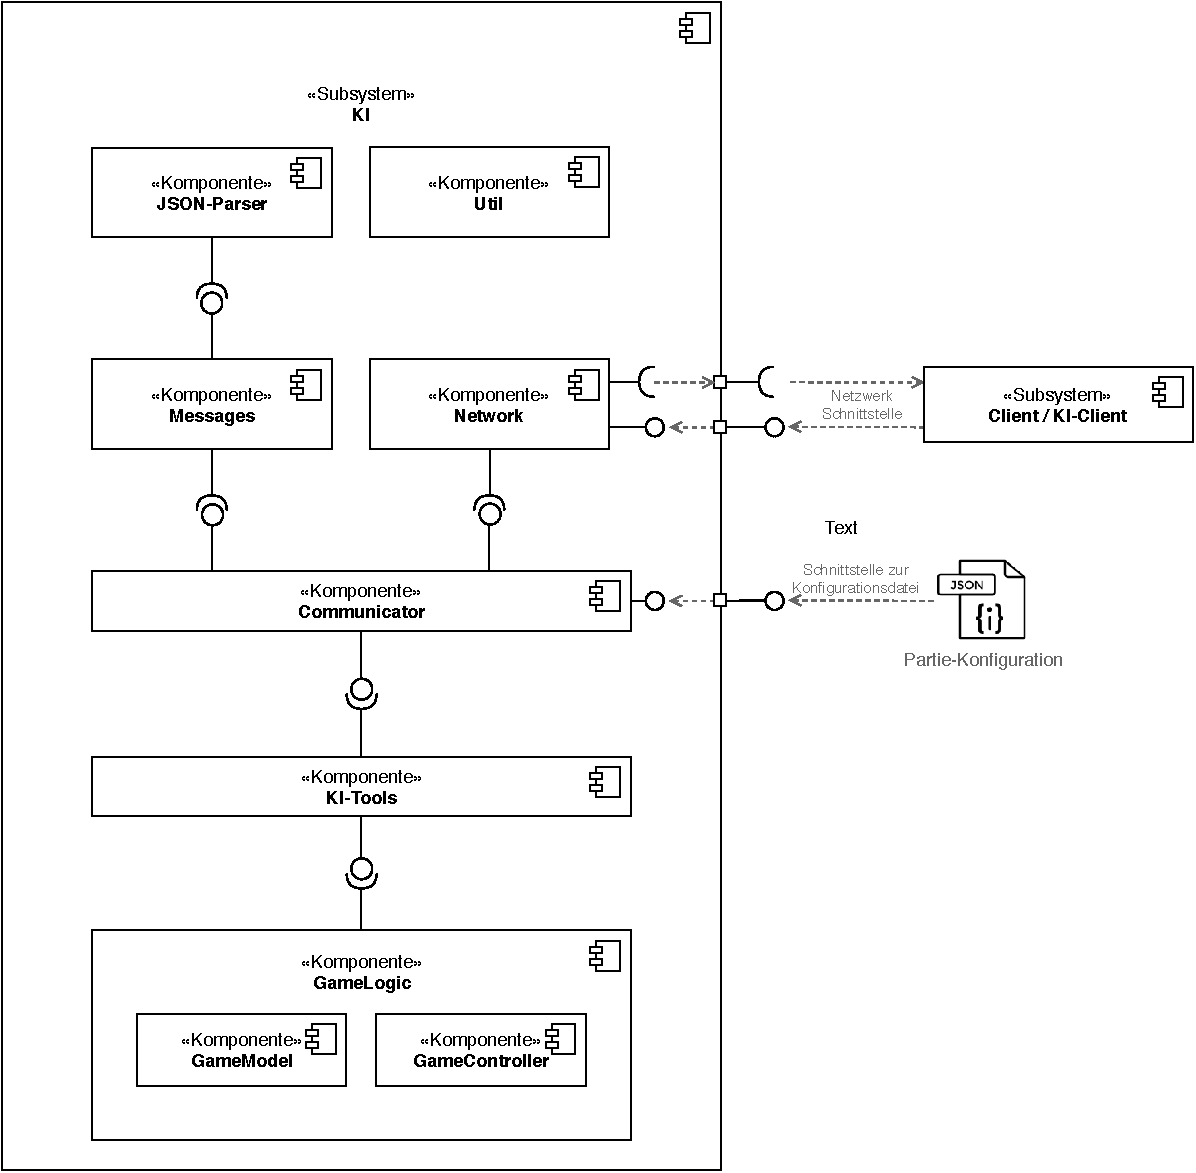
\includegraphics[scale=0.85]{../Endabnahme/images/KiDiagramme.pdf}
\end{figure}
    
\end{document}
